\documentclass[1p]{elsarticle_modified}
%\bibliographystyle{elsarticle-num}

%\usepackage[colorlinks]{hyperref}
%\usepackage{abbrmath_seonhwa} %\Abb, \Ascr, \Acal ,\Abf, \Afrak
\usepackage{amsfonts}
\usepackage{amssymb}
\usepackage{amsmath}
\usepackage{amsthm}
\usepackage{scalefnt}
\usepackage{amsbsy}
\usepackage{kotex}
\usepackage{caption}
\usepackage{subfig}
\usepackage{color}
\usepackage{graphicx}
\usepackage{xcolor} %% white, black, red, green, blue, cyan, magenta, yellow
\usepackage{float}
\usepackage{setspace}
\usepackage{hyperref}

\usepackage{tikz}
\usetikzlibrary{arrows}

\usepackage{multirow}
\usepackage{array} % fixed length table
\usepackage{hhline}

%%%%%%%%%%%%%%%%%%%%%
\makeatletter
\renewcommand*\env@matrix[1][\arraystretch]{%
	\edef\arraystretch{#1}%
	\hskip -\arraycolsep
	\let\@ifnextchar\new@ifnextchar
	\array{*\c@MaxMatrixCols c}}
\makeatother %https://tex.stackexchange.com/questions/14071/how-can-i-increase-the-line-spacing-in-a-matrix
%%%%%%%%%%%%%%%

\usepackage[normalem]{ulem}

\newcommand{\msout}[1]{\ifmmode\text{\sout{\ensuremath{#1}}}\else\sout{#1}\fi}
%SOURCE: \msout is \stkout macro in https://tex.stackexchange.com/questions/20609/strikeout-in-math-mode

\newcommand{\cancel}[1]{
	\ifmmode
	{\color{red}\msout{#1}}
	\else
	{\color{red}\sout{#1}}
	\fi
}

\newcommand{\add}[1]{
	{\color{blue}\uwave{#1}}
}

\newcommand{\replace}[2]{
	\ifmmode
	{\color{red}\msout{#1}}{\color{blue}\uwave{#2}}
	\else
	{\color{red}\sout{#1}}{\color{blue}\uwave{#2}}
	\fi
}

\newcommand{\Sol}{\mathcal{S}} %segment
\newcommand{\D}{D} %diagram
\newcommand{\A}{\mathcal{A}} %arc


%%%%%%%%%%%%%%%%%%%%%%%%%%%%%5 test

\def\sl{\operatorname{\textup{SL}}(2,\Cbb)}
\def\psl{\operatorname{\textup{PSL}}(2,\Cbb)}
\def\quan{\mkern 1mu \triangleright \mkern 1mu}

\theoremstyle{definition}
\newtheorem{thm}{Theorem}[section]
\newtheorem{prop}[thm]{Proposition}
\newtheorem{lem}[thm]{Lemma}
\newtheorem{ques}[thm]{Question}
\newtheorem{cor}[thm]{Corollary}
\newtheorem{defn}[thm]{Definition}
\newtheorem{exam}[thm]{Example}
\newtheorem{rmk}[thm]{Remark}
\newtheorem{alg}[thm]{Algorithm}

\newcommand{\I}{\sqrt{-1}}
\begin{document}

%\begin{frontmatter}
%
%\title{Boundary parabolic representations of knots up to 8 crossings}
%
%%% Group authors per affiliation:
%\author{Yunhi Cho} 
%\address{Department of Mathematics, University of Seoul, Seoul, Korea}
%\ead{yhcho@uos.ac.kr}
%
%
%\author{Seonhwa Kim} %\fnref{s_kim}}
%\address{Center for Geometry and Physics, Institute for Basic Science, Pohang, 37673, Korea}
%\ead{ryeona17@ibs.re.kr}
%
%\author{Hyuk Kim}
%\address{Department of Mathematical Sciences, Seoul National University, Seoul 08826, Korea}
%\ead{hyukkim@snu.ac.kr}
%
%\author{Seokbeom Yoon}
%\address{Department of Mathematical Sciences, Seoul National University, Seoul, 08826,  Korea}
%\ead{sbyoon15@snu.ac.kr}
%
%\begin{abstract}
%We find all boundary parabolic representation of knots up to 8 crossings.
%
%\end{abstract}
%\begin{keyword}
%    \MSC[2010] 57M25 
%\end{keyword}
%
%\end{frontmatter}

%\linenumbers
%\tableofcontents
%
\newcommand\colored[1]{\textcolor{white}{\rule[-0.35ex]{0.8em}{1.4ex}}\kern-0.8em\color{red} #1}%
%\newcommand\colored[1]{\textcolor{white}{ #1}\kern-2.17ex	\textcolor{white}{ #1}\kern-1.81ex	\textcolor{white}{ #1}\kern-2.15ex\color{red}#1	}

{\Large $\underline{12a_{0228}~(K12a_{0228})}$}

\setlength{\tabcolsep}{10pt}
\renewcommand{\arraystretch}{1.6}
\vspace{1cm}\begin{tabular}{m{100pt}>{\centering\arraybackslash}m{274pt}}
\multirow{5}{120pt}{
	\centering
	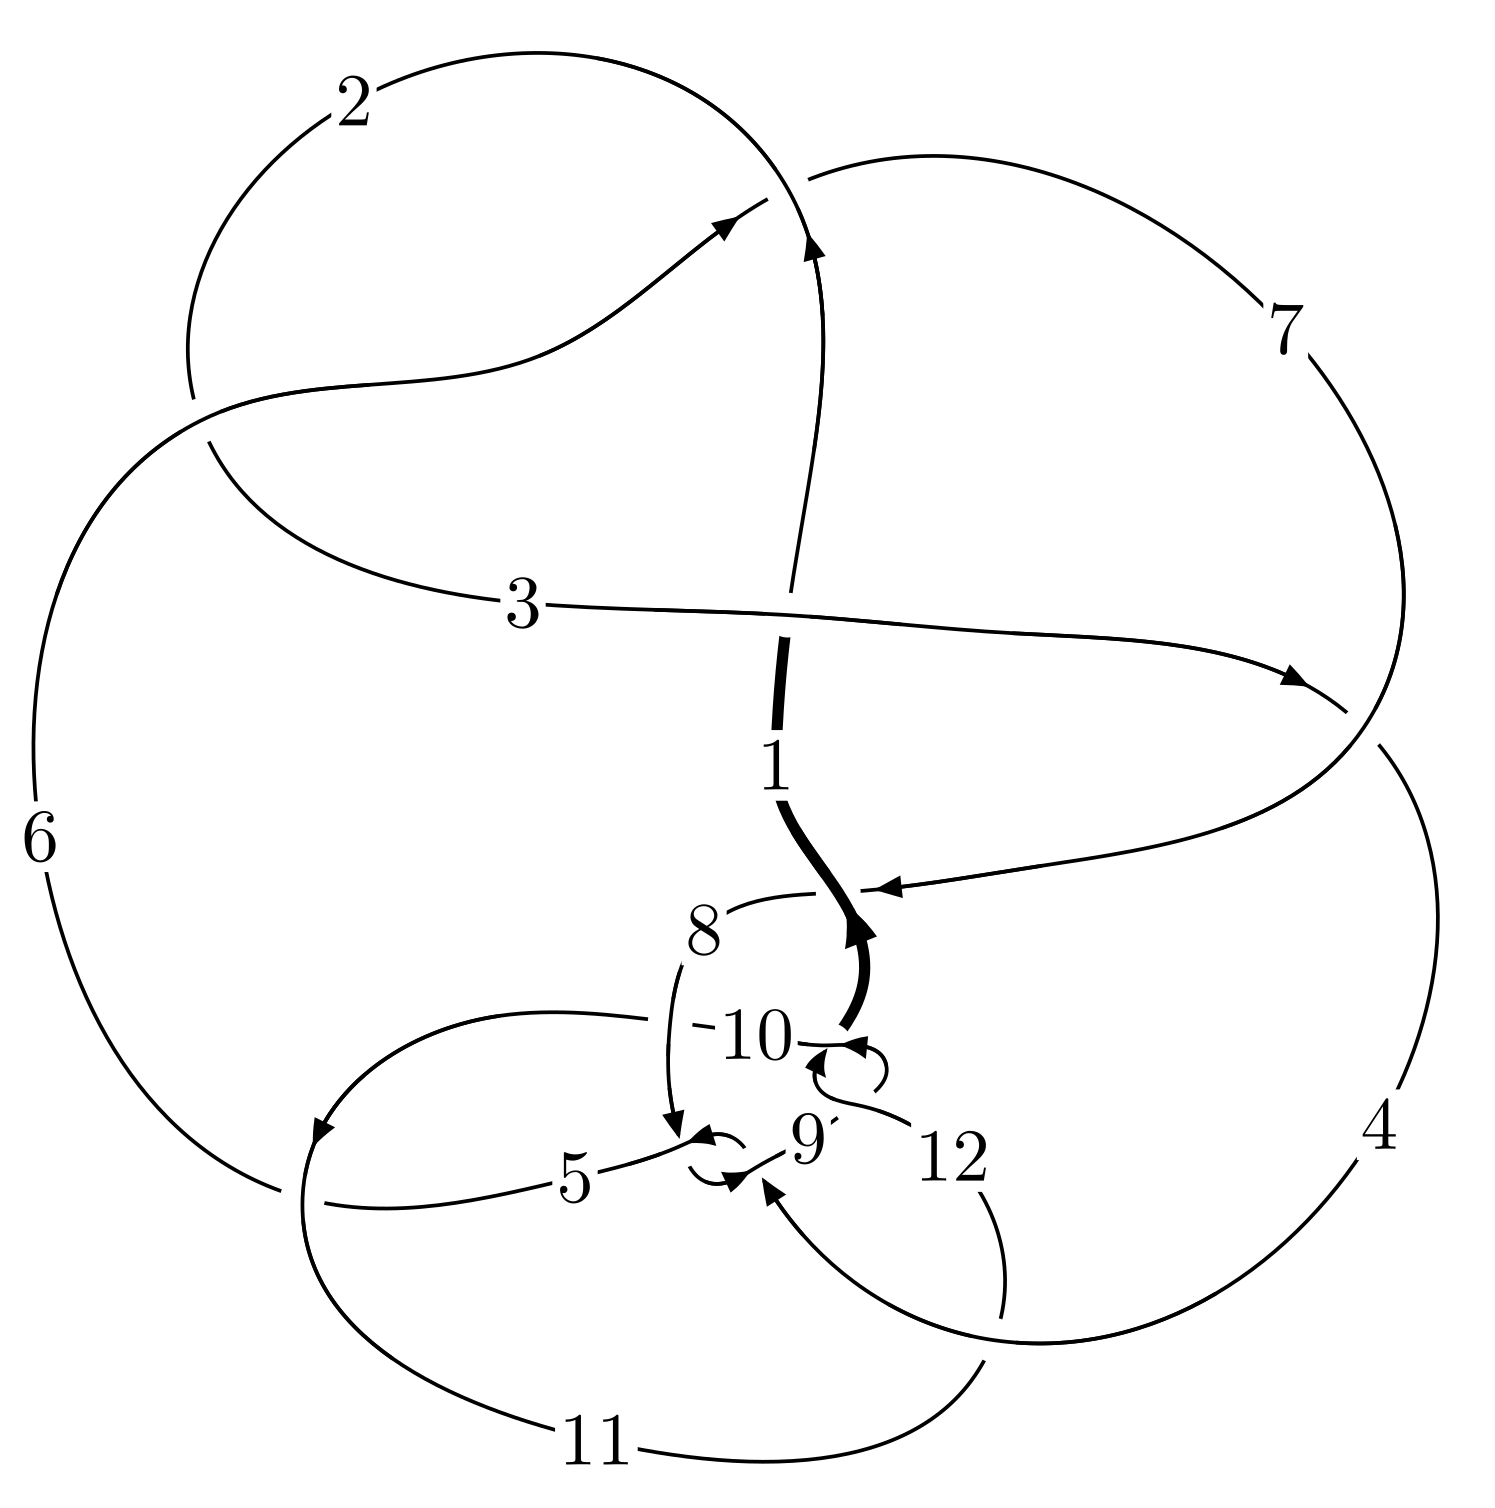
\includegraphics[width=112pt]{../../../GIT/diagram.site/Diagrams/png/1029_12a_0228.png}\\
\ \ \ A knot diagram\footnotemark}&
\allowdisplaybreaks
\textbf{Linearized knot diagam} \\
\cline{2-2}
 &
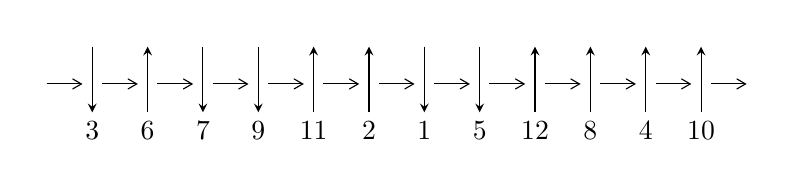
\begin{tikzpicture}[x=20pt, y=17pt]
	% nodes
	\node (C0) at (0, 0) {};
	\node (C1) at (1, 0) {};
	\node (C1U) at (1, +1) {};
	\node (C1D) at (1, -1) {3};

	\node (C2) at (2, 0) {};
	\node (C2U) at (2, +1) {};
	\node (C2D) at (2, -1) {6};

	\node (C3) at (3, 0) {};
	\node (C3U) at (3, +1) {};
	\node (C3D) at (3, -1) {7};

	\node (C4) at (4, 0) {};
	\node (C4U) at (4, +1) {};
	\node (C4D) at (4, -1) {9};

	\node (C5) at (5, 0) {};
	\node (C5U) at (5, +1) {};
	\node (C5D) at (5, -1) {11};

	\node (C6) at (6, 0) {};
	\node (C6U) at (6, +1) {};
	\node (C6D) at (6, -1) {2};

	\node (C7) at (7, 0) {};
	\node (C7U) at (7, +1) {};
	\node (C7D) at (7, -1) {1};

	\node (C8) at (8, 0) {};
	\node (C8U) at (8, +1) {};
	\node (C8D) at (8, -1) {5};

	\node (C9) at (9, 0) {};
	\node (C9U) at (9, +1) {};
	\node (C9D) at (9, -1) {12};

	\node (C10) at (10, 0) {};
	\node (C10U) at (10, +1) {};
	\node (C10D) at (10, -1) {8};

	\node (C11) at (11, 0) {};
	\node (C11U) at (11, +1) {};
	\node (C11D) at (11, -1) {4};

	\node (C12) at (12, 0) {};
	\node (C12U) at (12, +1) {};
	\node (C12D) at (12, -1) {10};
	\node (C13) at (13, 0) {};

	% arrows
	\draw[->,>={angle 60}]
	(C0) edge (C1) (C1) edge (C2) (C2) edge (C3) (C3) edge (C4) (C4) edge (C5) (C5) edge (C6) (C6) edge (C7) (C7) edge (C8) (C8) edge (C9) (C9) edge (C10) (C10) edge (C11) (C11) edge (C12) (C12) edge (C13) ;	\draw[->,>=stealth]
	(C1U) edge (C1D) (C2D) edge (C2U) (C3U) edge (C3D) (C4U) edge (C4D) (C5D) edge (C5U) (C6D) edge (C6U) (C7U) edge (C7D) (C8U) edge (C8D) (C9D) edge (C9U) (C10D) edge (C10U) (C11D) edge (C11U) (C12D) edge (C12U) ;
	\end{tikzpicture} \\
\hhline{~~} \\& 
\textbf{Solving Sequence} \\ \cline{2-2} 
 &
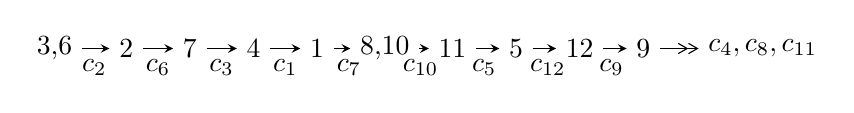
\begin{tikzpicture}[x=23pt, y=7pt]
	% node
	\node (A0) at (-1/8, 0) {3,6};
	\node (A1) at (1, 0) {2};
	\node (A2) at (2, 0) {7};
	\node (A3) at (3, 0) {4};
	\node (A4) at (4, 0) {1};
	\node (A5) at (81/16, 0) {8,10};
	\node (A6) at (49/8, 0) {11};
	\node (A7) at (57/8, 0) {5};
	\node (A8) at (65/8, 0) {12};
	\node (A9) at (73/8, 0) {9};
	\node (C1) at (1/2, -1) {$c_{2}$};
	\node (C2) at (3/2, -1) {$c_{6}$};
	\node (C3) at (5/2, -1) {$c_{3}$};
	\node (C4) at (7/2, -1) {$c_{1}$};
	\node (C5) at (9/2, -1) {$c_{7}$};
	\node (C6) at (45/8, -1) {$c_{10}$};
	\node (C7) at (53/8, -1) {$c_{5}$};
	\node (C8) at (61/8, -1) {$c_{12}$};
	\node (C9) at (69/8, -1) {$c_{9}$};
	\node (A10) at (11, 0) {$c_{4},c_{8},c_{11}$};

	% edge
	\draw[->,>=stealth]	
	(A0) edge (A1) (A1) edge (A2) (A2) edge (A3) (A3) edge (A4) (A4) edge (A5) (A5) edge (A6) (A6) edge (A7) (A7) edge (A8) (A8) edge (A9) ;
	\draw[->>,>={angle 60}]	
	(A9) edge (A10);
\end{tikzpicture} \\ 

\end{tabular} \\

\footnotetext{
The image of knot diagram is generated by the software ``\textbf{Draw programme}" developed by Andrew Bartholomew(\url{http://www.layer8.co.uk/maths/draw/index.htm\#Running-draw}), where we modified some parts for our purpose(\url{https://github.com/CATsTAILs/LinksPainter}).
}\phantom \\ \newline 
\centering \textbf{Ideals for irreducible components\footnotemark of $X_{\text{par}}$} 
 
\begin{align*}
I^u_{1}&=\langle 
5.75581\times10^{60} u^{115}+1.98417\times10^{61} u^{114}+\cdots+6.45264\times10^{60} b-1.60343\times10^{61},\\
\phantom{I^u_{1}}&\phantom{= \langle  }5.07246\times10^{60} u^{115}+7.72531\times10^{60} u^{114}+\cdots+2.15088\times10^{60} a-6.26357\times10^{60},\;u^{116}+2 u^{115}+\cdots-5 u-1\rangle \\
I^u_{2}&=\langle 
6 u^4-24 u^3+33 u^2+17 b-20 u-2,\;u^4-4 u^3+14 u^2+17 a-9 u+11,\;u^5- u^4+2 u^3- u^2+u-1\rangle \\
\\
\end{align*}
\raggedright * 2 irreducible components of $\dim_{\mathbb{C}}=0$, with total 121 representations.\\
\footnotetext{All coefficients of polynomials are rational numbers. But the coefficients are sometimes approximated in decimal forms when there is not enough margin.}
\newpage
\renewcommand{\arraystretch}{1}
\centering \section*{I. $I^u_{1}= \langle 5.76\times10^{60} u^{115}+1.98\times10^{61} u^{114}+\cdots+6.45\times10^{60} b-1.60\times10^{61},\;5.07\times10^{60} u^{115}+7.73\times10^{60} u^{114}+\cdots+2.15\times10^{60} a-6.26\times10^{60},\;u^{116}+2 u^{115}+\cdots-5 u-1 \rangle$}
\flushleft \textbf{(i) Arc colorings}\\
\begin{tabular}{m{7pt} m{180pt} m{7pt} m{180pt} }
\flushright $a_{3}=$&$\begin{pmatrix}1\\0\end{pmatrix}$ \\
\flushright $a_{6}=$&$\begin{pmatrix}0\\u\end{pmatrix}$ \\
\flushright $a_{2}=$&$\begin{pmatrix}1\\u^2\end{pmatrix}$ \\
\flushright $a_{7}=$&$\begin{pmatrix}u\\u^3+u\end{pmatrix}$ \\
\flushright $a_{4}=$&$\begin{pmatrix}u^4+u^2+1\\u^6+2 u^4+u^2\end{pmatrix}$ \\
\flushright $a_{1}=$&$\begin{pmatrix}u^2+1\\u^2\end{pmatrix}$ \\
\flushright $a_{8}=$&$\begin{pmatrix}- u^7-2 u^5-2 u^3\\- u^7- u^5+u\end{pmatrix}$ \\
\flushright $a_{10}=$&$\begin{pmatrix}-2.35832 u^{115}-3.59170 u^{114}+\cdots+5.62431 u+2.91210\\-0.892009 u^{115}-3.07497 u^{114}+\cdots+6.78907 u+2.48492\end{pmatrix}$ \\
\flushright $a_{11}=$&$\begin{pmatrix}-0.666357 u^{115}-0.411615 u^{114}+\cdots-1.02339 u+1.71894\\0.244543 u^{115}-0.720314 u^{114}+\cdots+1.56448 u+1.23807\end{pmatrix}$ \\
\flushright $a_{5}=$&$\begin{pmatrix}-2.30584 u^{115}-3.63509 u^{114}+\cdots+5.89997 u+2.09097\\-0.964992 u^{115}-1.49301 u^{114}+\cdots+3.05675 u+0.534737\end{pmatrix}$ \\
\flushright $a_{12}=$&$\begin{pmatrix}-2.56113 u^{115}-3.41397 u^{114}+\cdots+3.10597 u+3.15038\\-0.809371 u^{115}-2.81370 u^{114}+\cdots+6.08982 u+2.24085\end{pmatrix}$ \\
\flushright $a_{9}=$&$\begin{pmatrix}-0.00487807 u^{115}-1.44058 u^{114}+\cdots+9.57972 u+1.72391\\-0.539615 u^{115}-1.54506 u^{114}+\cdots+5.14801 u+1.34085\end{pmatrix}$\\&\end{tabular}
\flushleft \textbf{(ii) Obstruction class $= -1$}\\~\\
\flushleft \textbf{(iii) Cusp Shapes $= 4.97176 u^{115}+8.14134 u^{114}+\cdots-7.30434 u+7.67511$}\\~\\
\newpage\renewcommand{\arraystretch}{1}
\flushleft \textbf{(iv) u-Polynomials at the component}\newline \\
\begin{tabular}{m{50pt}|m{274pt}}
Crossings & \hspace{64pt}u-Polynomials at each crossing \\
\hline $$\begin{aligned}c_{1}\end{aligned}$$&$\begin{aligned}
&u^{116}+54 u^{115}+\cdots-11 u+1
\end{aligned}$\\
\hline $$\begin{aligned}c_{2},c_{6}\end{aligned}$$&$\begin{aligned}
&u^{116}-2 u^{115}+\cdots+5 u-1
\end{aligned}$\\
\hline $$\begin{aligned}c_{3}\end{aligned}$$&$\begin{aligned}
&u^{116}+2 u^{115}+\cdots+35 u-425
\end{aligned}$\\
\hline $$\begin{aligned}c_{4},c_{8}\end{aligned}$$&$\begin{aligned}
&u^{116}+2 u^{115}+\cdots+u-1
\end{aligned}$\\
\hline $$\begin{aligned}c_{5}\end{aligned}$$&$\begin{aligned}
&u^{116}+u^{115}+\cdots-76160 u+9248
\end{aligned}$\\
\hline $$\begin{aligned}c_{7}\end{aligned}$$&$\begin{aligned}
&u^{116}-10 u^{115}+\cdots+3962235 u-436275
\end{aligned}$\\
\hline $$\begin{aligned}c_{9},c_{12}\end{aligned}$$&$\begin{aligned}
&u^{116}+6 u^{115}+\cdots+3349 u-289
\end{aligned}$\\
\hline $$\begin{aligned}c_{10}\end{aligned}$$&$\begin{aligned}
&17(17 u^{116}-49 u^{115}+\cdots+4.80276\times10^{8} u+5.07692\times10^{7})
\end{aligned}$\\
\hline $$\begin{aligned}c_{11}\end{aligned}$$&$\begin{aligned}
&17(17 u^{116}+127 u^{115}+\cdots-6.60670\times10^{8} u+1.85956\times10^{8})
\end{aligned}$\\
\hline
\end{tabular}\\~\\
\newpage\renewcommand{\arraystretch}{1}
\flushleft \textbf{(v) Riley Polynomials at the component}\newline \\
\begin{tabular}{m{50pt}|m{274pt}}
Crossings & \hspace{64pt}Riley Polynomials at each crossing \\
\hline $$\begin{aligned}c_{1}\end{aligned}$$&$\begin{aligned}
&y^{116}+18 y^{115}+\cdots-203 y+1
\end{aligned}$\\
\hline $$\begin{aligned}c_{2},c_{6}\end{aligned}$$&$\begin{aligned}
&y^{116}+54 y^{115}+\cdots-11 y+1
\end{aligned}$\\
\hline $$\begin{aligned}c_{3}\end{aligned}$$&$\begin{aligned}
&y^{116}-18 y^{115}+\cdots-14809075 y+180625
\end{aligned}$\\
\hline $$\begin{aligned}c_{4},c_{8}\end{aligned}$$&$\begin{aligned}
&y^{116}+78 y^{115}+\cdots-11 y+1
\end{aligned}$\\
\hline $$\begin{aligned}c_{5}\end{aligned}$$&$\begin{aligned}
&y^{116}-33 y^{115}+\cdots-5184058880 y+85525504
\end{aligned}$\\
\hline $$\begin{aligned}c_{7}\end{aligned}$$&$\begin{aligned}
&y^{116}+54 y^{115}+\cdots+2904898639725 y+190335875625
\end{aligned}$\\
\hline $$\begin{aligned}c_{9},c_{12}\end{aligned}$$&$\begin{aligned}
&y^{116}-94 y^{115}+\cdots-10562661 y+83521
\end{aligned}$\\
\hline $$\begin{aligned}c_{10}\end{aligned}$$&$\begin{aligned}
&289(289 y^{116}-735 y^{115}+\cdots-8.40142\times10^{16} y+2.57752\times10^{15})
\end{aligned}$\\
\hline $$\begin{aligned}c_{11}\end{aligned}$$&$\begin{aligned}
&289(289 y^{116}-35645 y^{115}+\cdots-9.53692\times10^{17} y+3.45798\times10^{16})
\end{aligned}$\\
\hline
\end{tabular}\\~\\
\newpage\flushleft \textbf{(vi) Complex Volumes and Cusp Shapes}
$$\begin{array}{c|c|c}  
\text{Solutions to }I^u_{1}& \I (\text{vol} + \sqrt{-1}CS) & \text{Cusp shape}\\
 \hline 
\begin{aligned}
u &= -0.213726 + 0.979678 I \\
a &= \phantom{-}1.60090 + 0.53449 I \\
b &= \phantom{-}1.83411 - 0.89425 I\end{aligned}
 & \phantom{-}0.167995 + 0.526081 I & \phantom{-0.000000 } 0 \\ \hline\begin{aligned}
u &= -0.213726 - 0.979678 I \\
a &= \phantom{-}1.60090 - 0.53449 I \\
b &= \phantom{-}1.83411 + 0.89425 I\end{aligned}
 & \phantom{-}0.167995 - 0.526081 I & \phantom{-0.000000 } 0 \\ \hline\begin{aligned}
u &= \phantom{-}0.125887 + 0.978569 I \\
a &= \phantom{-}1.70020 - 0.61531 I \\
b &= \phantom{-}1.366030 + 0.140718 I\end{aligned}
 & \phantom{-}4.35805 - 1.96715 I & \phantom{-0.000000 } 0 \\ \hline\begin{aligned}
u &= \phantom{-}0.125887 - 0.978569 I \\
a &= \phantom{-}1.70020 + 0.61531 I \\
b &= \phantom{-}1.366030 - 0.140718 I\end{aligned}
 & \phantom{-}4.35805 + 1.96715 I & \phantom{-0.000000 } 0 \\ \hline\begin{aligned}
u &= \phantom{-}0.309540 + 0.933467 I \\
a &= \phantom{-}0.112007 - 0.737693 I \\
b &= \phantom{-}1.93325 - 1.81475 I\end{aligned}
 & \phantom{-}0.77750 + 1.28815 I & \phantom{-0.000000 } 0 \\ \hline\begin{aligned}
u &= \phantom{-}0.309540 - 0.933467 I \\
a &= \phantom{-}0.112007 + 0.737693 I \\
b &= \phantom{-}1.93325 + 1.81475 I\end{aligned}
 & \phantom{-}0.77750 - 1.28815 I & \phantom{-0.000000 } 0 \\ \hline\begin{aligned}
u &= \phantom{-}0.743846 + 0.630403 I \\
a &= \phantom{-}1.90685 + 1.03273 I \\
b &= -0.22355 + 1.92834 I\end{aligned}
 & \phantom{-}10.83050 - 1.67305 I & \phantom{-0.000000 } 0 \\ \hline\begin{aligned}
u &= \phantom{-}0.743846 - 0.630403 I \\
a &= \phantom{-}1.90685 - 1.03273 I \\
b &= -0.22355 - 1.92834 I\end{aligned}
 & \phantom{-}10.83050 + 1.67305 I & \phantom{-0.000000 } 0 \\ \hline\begin{aligned}
u &= -0.751758 + 0.607698 I \\
a &= \phantom{-}1.95762 - 1.27271 I \\
b &= -0.39410 - 1.79230 I\end{aligned}
 & \phantom{-}6.55718 - 4.78302 I & \phantom{-0.000000 } 0 \\ \hline\begin{aligned}
u &= -0.751758 - 0.607698 I \\
a &= \phantom{-}1.95762 + 1.27271 I \\
b &= -0.39410 + 1.79230 I\end{aligned}
 & \phantom{-}6.55718 + 4.78302 I & \phantom{-0.000000 } 0\\
 \hline 
 \end{array}$$\newpage$$\begin{array}{c|c|c}  
\text{Solutions to }I^u_{1}& \I (\text{vol} + \sqrt{-1}CS) & \text{Cusp shape}\\
 \hline 
\begin{aligned}
u &= \phantom{-}0.738019 + 0.605133 I \\
a &= \phantom{-}2.08860 + 1.33989 I \\
b &= -0.58143 + 1.83889 I\end{aligned}
 & \phantom{-}11.3529 + 10.6244 I & \phantom{-0.000000 } 0 \\ \hline\begin{aligned}
u &= \phantom{-}0.738019 - 0.605133 I \\
a &= \phantom{-}2.08860 - 1.33989 I \\
b &= -0.58143 - 1.83889 I\end{aligned}
 & \phantom{-}11.3529 - 10.6244 I & \phantom{-0.000000 } 0 \\ \hline\begin{aligned}
u &= -0.236713 + 1.018870 I \\
a &= \phantom{-}0.376854 - 0.678326 I \\
b &= -0.900450 - 1.066460 I\end{aligned}
 & -0.027406 - 1.051670 I & \phantom{-0.000000 } 0 \\ \hline\begin{aligned}
u &= -0.236713 - 1.018870 I \\
a &= \phantom{-}0.376854 + 0.678326 I \\
b &= -0.900450 + 1.066460 I\end{aligned}
 & -0.027406 + 1.051670 I & \phantom{-0.000000 } 0 \\ \hline\begin{aligned}
u &= \phantom{-}0.319760 + 1.015070 I \\
a &= -2.16164 + 3.60624 I \\
b &= -7.18790 - 1.77810 I\end{aligned}
 & \phantom{-}1.33619 + 0.84695 I & \phantom{-0.000000 } 0 \\ \hline\begin{aligned}
u &= \phantom{-}0.319760 - 1.015070 I \\
a &= -2.16164 - 3.60624 I \\
b &= -7.18790 + 1.77810 I\end{aligned}
 & \phantom{-}1.33619 - 0.84695 I & \phantom{-0.000000 } 0 \\ \hline\begin{aligned}
u &= \phantom{-}0.447876 + 0.971546 I \\
a &= -0.044939 + 1.030310 I \\
b &= -0.0173674 - 0.0369021 I\end{aligned}
 & \phantom{-}2.76198 + 4.91396 I & \phantom{-0.000000 } 0 \\ \hline\begin{aligned}
u &= \phantom{-}0.447876 - 0.971546 I \\
a &= -0.044939 - 1.030310 I \\
b &= -0.0173674 + 0.0369021 I\end{aligned}
 & \phantom{-}2.76198 - 4.91396 I & \phantom{-0.000000 } 0 \\ \hline\begin{aligned}
u &= -0.387226 + 0.997733 I \\
a &= -0.479626 - 0.904983 I \\
b &= -0.853551 + 0.688235 I\end{aligned}
 & -0.83470 - 2.75967 I & \phantom{-0.000000 } 0 \\ \hline\begin{aligned}
u &= -0.387226 - 0.997733 I \\
a &= -0.479626 + 0.904983 I \\
b &= -0.853551 - 0.688235 I\end{aligned}
 & -0.83470 + 2.75967 I & \phantom{-0.000000 } 0\\
 \hline 
 \end{array}$$\newpage$$\begin{array}{c|c|c}  
\text{Solutions to }I^u_{1}& \I (\text{vol} + \sqrt{-1}CS) & \text{Cusp shape}\\
 \hline 
\begin{aligned}
u &= -0.180477 + 1.077350 I \\
a &= \phantom{-}0.552778 + 1.052860 I \\
b &= \phantom{-}0.411909 - 0.007067 I\end{aligned}
 & -0.03499 + 4.92088 I & \phantom{-0.000000 } 0 \\ \hline\begin{aligned}
u &= -0.180477 - 1.077350 I \\
a &= \phantom{-}0.552778 - 1.052860 I \\
b &= \phantom{-}0.411909 + 0.007067 I\end{aligned}
 & -0.03499 - 4.92088 I & \phantom{-0.000000 } 0 \\ \hline\begin{aligned}
u &= -0.826428 + 0.374638 I \\
a &= \phantom{-}1.16217 - 2.07695 I \\
b &= -0.69074 - 1.49489 I\end{aligned}
 & \phantom{-}9.38100 + 1.35019 I & \phantom{-0.000000 } 0 \\ \hline\begin{aligned}
u &= -0.826428 - 0.374638 I \\
a &= \phantom{-}1.16217 + 2.07695 I \\
b &= -0.69074 + 1.49489 I\end{aligned}
 & \phantom{-}9.38100 - 1.35019 I & \phantom{-0.000000 } 0 \\ \hline\begin{aligned}
u &= -0.371827 + 0.824359 I \\
a &= \phantom{-}0.707381 - 0.378871 I \\
b &= \phantom{-}1.156950 + 0.662434 I\end{aligned}
 & \phantom{-}4.93896 - 1.72487 I & \phantom{-0.000000 } 0 \\ \hline\begin{aligned}
u &= -0.371827 - 0.824359 I \\
a &= \phantom{-}0.707381 + 0.378871 I \\
b &= \phantom{-}1.156950 - 0.662434 I\end{aligned}
 & \phantom{-}4.93896 + 1.72487 I & \phantom{-0.000000 } 0 \\ \hline\begin{aligned}
u &= \phantom{-}0.813710 + 0.390654 I \\
a &= \phantom{-}1.65938 + 2.30133 I \\
b &= -0.47737 + 1.91274 I\end{aligned}
 & \phantom{-}5.35441 - 7.81379 I & \phantom{-0.000000 } 0 \\ \hline\begin{aligned}
u &= \phantom{-}0.813710 - 0.390654 I \\
a &= \phantom{-}1.65938 - 2.30133 I \\
b &= -0.47737 - 1.91274 I\end{aligned}
 & \phantom{-}5.35441 + 7.81379 I & \phantom{-0.000000 } 0 \\ \hline\begin{aligned}
u &= \phantom{-}0.214588 + 1.080830 I \\
a &= \phantom{-}0.237087 - 0.533447 I \\
b &= \phantom{-}0.002009 + 0.228143 I\end{aligned}
 & -3.44211 - 1.31744 I & \phantom{-0.000000 } 0 \\ \hline\begin{aligned}
u &= \phantom{-}0.214588 - 1.080830 I \\
a &= \phantom{-}0.237087 + 0.533447 I \\
b &= \phantom{-}0.002009 - 0.228143 I\end{aligned}
 & -3.44211 + 1.31744 I & \phantom{-0.000000 } 0\\
 \hline 
 \end{array}$$\newpage$$\begin{array}{c|c|c}  
\text{Solutions to }I^u_{1}& \I (\text{vol} + \sqrt{-1}CS) & \text{Cusp shape}\\
 \hline 
\begin{aligned}
u &= -0.806147 + 0.384835 I \\
a &= \phantom{-}1.75293 - 2.64831 I \\
b &= -0.59316 - 2.20336 I\end{aligned}
 & \phantom{-}10.1438 + 13.5286 I & \phantom{-0.000000 } 0 \\ \hline\begin{aligned}
u &= -0.806147 - 0.384835 I \\
a &= \phantom{-}1.75293 + 2.64831 I \\
b &= -0.59316 + 2.20336 I\end{aligned}
 & \phantom{-}10.1438 - 13.5286 I & \phantom{-0.000000 } 0 \\ \hline\begin{aligned}
u &= \phantom{-}0.684803 + 0.538931 I \\
a &= \phantom{-}0.356592 - 0.731019 I \\
b &= \phantom{-}1.144010 + 0.473688 I\end{aligned}
 & \phantom{-}5.38099 + 4.74367 I & \phantom{-0.000000 } 0 \\ \hline\begin{aligned}
u &= \phantom{-}0.684803 - 0.538931 I \\
a &= \phantom{-}0.356592 + 0.731019 I \\
b &= \phantom{-}1.144010 - 0.473688 I\end{aligned}
 & \phantom{-}5.38099 - 4.74367 I & \phantom{-0.000000 } 0 \\ \hline\begin{aligned}
u &= -0.716074 + 0.485984 I \\
a &= -1.56043 + 1.94624 I \\
b &= \phantom{-}1.28088 + 1.50181 I\end{aligned}
 & \phantom{-}9.28238 - 1.11602 I & \phantom{-}13.84835 + 0. I\phantom{ +0.000000I} \\ \hline\begin{aligned}
u &= -0.716074 - 0.485984 I \\
a &= -1.56043 - 1.94624 I \\
b &= \phantom{-}1.28088 - 1.50181 I\end{aligned}
 & \phantom{-}9.28238 + 1.11602 I & \phantom{-}13.84835 + 0. I\phantom{ +0.000000I} \\ \hline\begin{aligned}
u &= \phantom{-}0.735710 + 0.444784 I \\
a &= -2.10447 - 2.13484 I \\
b &= \phantom{-}0.58715 - 2.40571 I\end{aligned}
 & \phantom{-}9.06427 - 3.60222 I & \phantom{-}13.25447 + 0. I\phantom{ +0.000000I} \\ \hline\begin{aligned}
u &= \phantom{-}0.735710 - 0.444784 I \\
a &= -2.10447 + 2.13484 I \\
b &= \phantom{-}0.58715 + 2.40571 I\end{aligned}
 & \phantom{-}9.06427 + 3.60222 I & \phantom{-}13.25447 + 0. I\phantom{ +0.000000I} \\ \hline\begin{aligned}
u &= -0.751426 + 0.398872 I \\
a &= -1.331980 + 0.280135 I \\
b &= -0.65647 + 1.33074 I\end{aligned}
 & \phantom{-}4.65190 + 7.12858 I & \phantom{-}8.00466 - 6.45034 I \\ \hline\begin{aligned}
u &= -0.751426 - 0.398872 I \\
a &= -1.331980 - 0.280135 I \\
b &= -0.65647 - 1.33074 I\end{aligned}
 & \phantom{-}4.65190 - 7.12858 I & \phantom{-}8.00466 + 6.45034 I\\
 \hline 
 \end{array}$$\newpage$$\begin{array}{c|c|c}  
\text{Solutions to }I^u_{1}& \I (\text{vol} + \sqrt{-1}CS) & \text{Cusp shape}\\
 \hline 
\begin{aligned}
u &= -0.158418 + 1.151430 I \\
a &= -1.74281 - 0.26217 I \\
b &= -1.73088 + 0.55675 I\end{aligned}
 & \phantom{-}5.05609 + 10.97800 I & \phantom{-0.000000 } 0 \\ \hline\begin{aligned}
u &= -0.158418 - 1.151430 I \\
a &= -1.74281 + 0.26217 I \\
b &= -1.73088 - 0.55675 I\end{aligned}
 & \phantom{-}5.05609 - 10.97800 I & \phantom{-0.000000 } 0 \\ \hline\begin{aligned}
u &= -0.407944 + 1.088610 I \\
a &= -0.970445 - 0.729417 I \\
b &= -0.746780 + 0.242375 I\end{aligned}
 & -2.10001 - 6.03359 I & \phantom{-0.000000 } 0 \\ \hline\begin{aligned}
u &= -0.407944 - 1.088610 I \\
a &= -0.970445 + 0.729417 I \\
b &= -0.746780 - 0.242375 I\end{aligned}
 & -2.10001 + 6.03359 I & \phantom{-0.000000 } 0 \\ \hline\begin{aligned}
u &= \phantom{-}0.647035 + 0.966883 I \\
a &= \phantom{-}0.60997 + 1.62296 I \\
b &= -1.15036 + 2.56312 I\end{aligned}
 & \phantom{-}9.82905 + 6.94446 I & \phantom{-0.000000 } 0 \\ \hline\begin{aligned}
u &= \phantom{-}0.647035 - 0.966883 I \\
a &= \phantom{-}0.60997 - 1.62296 I \\
b &= -1.15036 - 2.56312 I\end{aligned}
 & \phantom{-}9.82905 - 6.94446 I & \phantom{-0.000000 } 0 \\ \hline\begin{aligned}
u &= -0.644975 + 0.529795 I \\
a &= \phantom{-}0.317585 - 0.144452 I \\
b &= \phantom{-}0.444610 - 0.522513 I\end{aligned}
 & \phantom{-}1.80492 - 1.53618 I & \phantom{-}3.15801 + 3.61737 I \\ \hline\begin{aligned}
u &= -0.644975 - 0.529795 I \\
a &= \phantom{-}0.317585 + 0.144452 I \\
b &= \phantom{-}0.444610 + 0.522513 I\end{aligned}
 & \phantom{-}1.80492 + 1.53618 I & \phantom{-}3.15801 - 3.61737 I \\ \hline\begin{aligned}
u &= \phantom{-}0.689493 + 0.467421 I \\
a &= -2.87010 - 1.03664 I \\
b &= \phantom{-}0.09768 - 1.55760 I\end{aligned}
 & \phantom{-}4.67202 + 0.02612 I & \phantom{-}5.05104 + 0. I\phantom{ +0.000000I} \\ \hline\begin{aligned}
u &= \phantom{-}0.689493 - 0.467421 I \\
a &= -2.87010 + 1.03664 I \\
b &= \phantom{-}0.09768 + 1.55760 I\end{aligned}
 & \phantom{-}4.67202 - 0.02612 I & \phantom{-}5.05104 + 0. I\phantom{ +0.000000I}\\
 \hline 
 \end{array}$$\newpage$$\begin{array}{c|c|c}  
\text{Solutions to }I^u_{1}& \I (\text{vol} + \sqrt{-1}CS) & \text{Cusp shape}\\
 \hline 
\begin{aligned}
u &= -0.710222 + 0.434714 I \\
a &= -1.75555 + 2.99422 I \\
b &= \phantom{-}0.84628 + 2.17663 I\end{aligned}
 & \phantom{-}4.49672 + 2.23779 I & \phantom{-}5.47097 - 1.27314 I \\ \hline\begin{aligned}
u &= -0.710222 - 0.434714 I \\
a &= -1.75555 - 2.99422 I \\
b &= \phantom{-}0.84628 - 2.17663 I\end{aligned}
 & \phantom{-}4.49672 - 2.23779 I & \phantom{-}5.47097 + 1.27314 I \\ \hline\begin{aligned}
u &= \phantom{-}0.374555 + 1.106800 I \\
a &= -0.745632 + 0.391856 I \\
b &= -0.565566 - 0.009069 I\end{aligned}
 & -4.95014 + 1.97544 I & \phantom{-0.000000 } 0 \\ \hline\begin{aligned}
u &= \phantom{-}0.374555 - 1.106800 I \\
a &= -0.745632 - 0.391856 I \\
b &= -0.565566 + 0.009069 I\end{aligned}
 & -4.95014 - 1.97544 I & \phantom{-0.000000 } 0 \\ \hline\begin{aligned}
u &= \phantom{-}0.145684 + 1.159730 I \\
a &= -1.47907 + 0.20648 I \\
b &= -1.61847 - 0.35202 I\end{aligned}
 & \phantom{-}0.17052 - 5.27151 I & \phantom{-0.000000 } 0 \\ \hline\begin{aligned}
u &= \phantom{-}0.145684 - 1.159730 I \\
a &= -1.47907 - 0.20648 I \\
b &= -1.61847 + 0.35202 I\end{aligned}
 & \phantom{-}0.17052 + 5.27151 I & \phantom{-0.000000 } 0 \\ \hline\begin{aligned}
u &= -0.552992 + 1.030300 I \\
a &= \phantom{-}0.343583 - 0.419278 I \\
b &= -0.529664 - 0.227199 I\end{aligned}
 & \phantom{-}0.31815 - 3.15390 I & \phantom{-0.000000 } 0 \\ \hline\begin{aligned}
u &= -0.552992 - 1.030300 I \\
a &= \phantom{-}0.343583 + 0.419278 I \\
b &= -0.529664 + 0.227199 I\end{aligned}
 & \phantom{-}0.31815 + 3.15390 I & \phantom{-0.000000 } 0 \\ \hline\begin{aligned}
u &= -0.449021 + 1.080700 I \\
a &= \phantom{-}0.697371 - 0.733803 I \\
b &= -0.81172 - 1.64241 I\end{aligned}
 & -1.83928 - 1.16536 I & \phantom{-0.000000 } 0 \\ \hline\begin{aligned}
u &= -0.449021 - 1.080700 I \\
a &= \phantom{-}0.697371 + 0.733803 I \\
b &= -0.81172 + 1.64241 I\end{aligned}
 & -1.83928 + 1.16536 I & \phantom{-0.000000 } 0\\
 \hline 
 \end{array}$$\newpage$$\begin{array}{c|c|c}  
\text{Solutions to }I^u_{1}& \I (\text{vol} + \sqrt{-1}CS) & \text{Cusp shape}\\
 \hline 
\begin{aligned}
u &= \phantom{-}0.734193 + 0.382672 I \\
a &= -0.363486 - 0.221446 I \\
b &= -0.252124 - 0.679881 I\end{aligned}
 & \phantom{-}1.04420 - 3.63453 I & \phantom{-}2.00000 + 3.37564 I \\ \hline\begin{aligned}
u &= \phantom{-}0.734193 - 0.382672 I \\
a &= -0.363486 + 0.221446 I \\
b &= -0.252124 + 0.679881 I\end{aligned}
 & \phantom{-}1.04420 + 3.63453 I & \phantom{-}2.00000 - 3.37564 I \\ \hline\begin{aligned}
u &= \phantom{-}0.636595 + 0.984802 I \\
a &= \phantom{-}0.71956 + 1.68566 I \\
b &= -0.73241 + 2.95425 I\end{aligned}
 & \phantom{-}10.22580 - 5.40240 I & \phantom{-0.000000 } 0 \\ \hline\begin{aligned}
u &= \phantom{-}0.636595 - 0.984802 I \\
a &= \phantom{-}0.71956 - 1.68566 I \\
b &= -0.73241 - 2.95425 I\end{aligned}
 & \phantom{-}10.22580 + 5.40240 I & \phantom{-0.000000 } 0 \\ \hline\begin{aligned}
u &= \phantom{-}0.826337\phantom{ +0.000000I} \\
a &= \phantom{-}0.752087\phantom{ +0.000000I} \\
b &= -0.356164\phantom{ +0.000000I}\end{aligned}
 & -0.424621\phantom{ +0.000000I} & \phantom{-}19.7700\phantom{ +0.000000I} \\ \hline\begin{aligned}
u &= \phantom{-}0.578311 + 1.021470 I \\
a &= -0.325740 + 0.405044 I \\
b &= -1.47077 - 0.57548 I\end{aligned}
 & \phantom{-}3.95182 + 0.14125 I & \phantom{-0.000000 } 0 \\ \hline\begin{aligned}
u &= \phantom{-}0.578311 - 1.021470 I \\
a &= -0.325740 - 0.405044 I \\
b &= -1.47077 + 0.57548 I\end{aligned}
 & \phantom{-}3.95182 - 0.14125 I & \phantom{-0.000000 } 0 \\ \hline\begin{aligned}
u &= -0.648829 + 0.986349 I \\
a &= \phantom{-}0.69438 - 1.65109 I \\
b &= -0.81010 - 2.70604 I\end{aligned}
 & \phantom{-}5.43273 - 0.51549 I & \phantom{-0.000000 } 0 \\ \hline\begin{aligned}
u &= -0.648829 - 0.986349 I \\
a &= \phantom{-}0.69438 + 1.65109 I \\
b &= -0.81010 + 2.70604 I\end{aligned}
 & \phantom{-}5.43273 + 0.51549 I & \phantom{-0.000000 } 0 \\ \hline\begin{aligned}
u &= -0.341593 + 0.739889 I \\
a &= \phantom{-}0.491846 - 0.519334 I \\
b &= -0.650693 - 0.657690 I\end{aligned}
 & -0.07351 - 1.53899 I & -0.35735 + 4.62669 I\\
 \hline 
 \end{array}$$\newpage$$\begin{array}{c|c|c}  
\text{Solutions to }I^u_{1}& \I (\text{vol} + \sqrt{-1}CS) & \text{Cusp shape}\\
 \hline 
\begin{aligned}
u &= -0.341593 - 0.739889 I \\
a &= \phantom{-}0.491846 + 0.519334 I \\
b &= -0.650693 + 0.657690 I\end{aligned}
 & -0.07351 + 1.53899 I & -0.35735 - 4.62669 I \\ \hline\begin{aligned}
u &= -0.702246 + 0.400107 I \\
a &= \phantom{-}1.66196 + 0.97308 I \\
b &= \phantom{-}1.088350 + 0.037803 I\end{aligned}
 & \phantom{-}4.18759 + 0.99207 I & \phantom{-}8.76986 + 0. I\phantom{ +0.000000I} \\ \hline\begin{aligned}
u &= -0.702246 - 0.400107 I \\
a &= \phantom{-}1.66196 - 0.97308 I \\
b &= \phantom{-}1.088350 - 0.037803 I\end{aligned}
 & \phantom{-}4.18759 - 0.99207 I & \phantom{-}8.76986 + 0. I\phantom{ +0.000000I} \\ \hline\begin{aligned}
u &= \phantom{-}0.551493 + 1.056650 I \\
a &= \phantom{-}2.34626 + 0.85733 I \\
b &= \phantom{-}1.41245 + 2.07391 I\end{aligned}
 & \phantom{-}2.91340 + 5.62132 I & \phantom{-0.000000 } 0 \\ \hline\begin{aligned}
u &= \phantom{-}0.551493 - 1.056650 I \\
a &= \phantom{-}2.34626 - 0.85733 I \\
b &= \phantom{-}1.41245 - 2.07391 I\end{aligned}
 & \phantom{-}2.91340 - 5.62132 I & \phantom{-0.000000 } 0 \\ \hline\begin{aligned}
u &= -0.170661 + 1.184020 I \\
a &= -1.317040 + 0.124672 I \\
b &= -1.237580 + 0.310417 I\end{aligned}
 & \phantom{-}4.20227 - 1.40731 I & \phantom{-0.000000 } 0 \\ \hline\begin{aligned}
u &= -0.170661 - 1.184020 I \\
a &= -1.317040 - 0.124672 I \\
b &= -1.237580 - 0.310417 I\end{aligned}
 & \phantom{-}4.20227 + 1.40731 I & \phantom{-0.000000 } 0 \\ \hline\begin{aligned}
u &= \phantom{-}0.637926 + 0.481213 I \\
a &= \phantom{-}0.31869 + 2.12232 I \\
b &= -0.247274 + 0.566263 I\end{aligned}
 & \phantom{-}4.62411 - 0.94935 I & \phantom{-}11.70670 + 0.13383 I \\ \hline\begin{aligned}
u &= \phantom{-}0.637926 - 0.481213 I \\
a &= \phantom{-}0.31869 - 2.12232 I \\
b &= -0.247274 - 0.566263 I\end{aligned}
 & \phantom{-}4.62411 + 0.94935 I & \phantom{-}11.70670 - 0.13383 I \\ \hline\begin{aligned}
u &= \phantom{-}0.573566 + 1.061840 I \\
a &= -0.29785 - 2.25510 I \\
b &= \phantom{-}1.55526 - 3.19666 I\end{aligned}
 & \phantom{-}2.91832 + 4.85580 I & \phantom{-0.000000 } 0\\
 \hline 
 \end{array}$$\newpage$$\begin{array}{c|c|c}  
\text{Solutions to }I^u_{1}& \I (\text{vol} + \sqrt{-1}CS) & \text{Cusp shape}\\
 \hline 
\begin{aligned}
u &= \phantom{-}0.573566 - 1.061840 I \\
a &= -0.29785 + 2.25510 I \\
b &= \phantom{-}1.55526 + 3.19666 I\end{aligned}
 & \phantom{-}2.91832 - 4.85580 I & \phantom{-0.000000 } 0 \\ \hline\begin{aligned}
u &= -0.589394 + 1.056650 I \\
a &= -1.20022 + 1.15722 I \\
b &= -0.28853 + 3.39941 I\end{aligned}
 & \phantom{-}7.59396 - 3.88847 I & \phantom{-0.000000 } 0 \\ \hline\begin{aligned}
u &= -0.589394 - 1.056650 I \\
a &= -1.20022 - 1.15722 I \\
b &= -0.28853 - 3.39941 I\end{aligned}
 & \phantom{-}7.59396 + 3.88847 I & \phantom{-0.000000 } 0 \\ \hline\begin{aligned}
u &= \phantom{-}0.476904 + 1.120410 I \\
a &= \phantom{-}0.501150 + 0.454538 I \\
b &= -0.31692 + 1.52578 I\end{aligned}
 & -4.25414 + 5.60705 I & \phantom{-0.000000 } 0 \\ \hline\begin{aligned}
u &= \phantom{-}0.476904 - 1.120410 I \\
a &= \phantom{-}0.501150 - 0.454538 I \\
b &= -0.31692 - 1.52578 I\end{aligned}
 & -4.25414 - 5.60705 I & \phantom{-0.000000 } 0 \\ \hline\begin{aligned}
u &= -0.577539 + 1.078690 I \\
a &= -2.11320 + 1.66372 I \\
b &= -0.17083 + 4.02607 I\end{aligned}
 & \phantom{-}2.60273 - 7.18374 I & \phantom{-0.000000 } 0 \\ \hline\begin{aligned}
u &= -0.577539 - 1.078690 I \\
a &= -2.11320 - 1.66372 I \\
b &= -0.17083 - 4.02607 I\end{aligned}
 & \phantom{-}2.60273 + 7.18374 I & \phantom{-0.000000 } 0 \\ \hline\begin{aligned}
u &= -0.566964 + 1.089470 I \\
a &= -1.05362 - 1.05257 I \\
b &= -1.68561 + 0.12365 I\end{aligned}
 & \phantom{-}2.17207 - 5.87574 I & \phantom{-0.000000 } 0 \\ \hline\begin{aligned}
u &= -0.566964 - 1.089470 I \\
a &= -1.05362 + 1.05257 I \\
b &= -1.68561 - 0.12365 I\end{aligned}
 & \phantom{-}2.17207 + 5.87574 I & \phantom{-0.000000 } 0 \\ \hline\begin{aligned}
u &= \phantom{-}0.589893 + 1.079910 I \\
a &= -1.51806 - 1.70782 I \\
b &= \phantom{-}0.76044 - 3.88756 I\end{aligned}
 & \phantom{-}7.18842 + 8.65606 I & \phantom{-0.000000 } 0\\
 \hline 
 \end{array}$$\newpage$$\begin{array}{c|c|c}  
\text{Solutions to }I^u_{1}& \I (\text{vol} + \sqrt{-1}CS) & \text{Cusp shape}\\
 \hline 
\begin{aligned}
u &= \phantom{-}0.589893 - 1.079910 I \\
a &= -1.51806 + 1.70782 I \\
b &= \phantom{-}0.76044 + 3.88756 I\end{aligned}
 & \phantom{-}7.18842 - 8.65606 I & \phantom{-0.000000 } 0 \\ \hline\begin{aligned}
u &= -0.402416 + 1.170640 I \\
a &= -0.558708 + 0.087620 I \\
b &= -0.013361 - 0.491838 I\end{aligned}
 & \phantom{-}1.32732 + 2.51230 I & \phantom{-0.000000 } 0 \\ \hline\begin{aligned}
u &= -0.402416 - 1.170640 I \\
a &= -0.558708 - 0.087620 I \\
b &= -0.013361 + 0.491838 I\end{aligned}
 & \phantom{-}1.32732 - 2.51230 I & \phantom{-0.000000 } 0 \\ \hline\begin{aligned}
u &= -0.443018 + 1.159920 I \\
a &= \phantom{-}0.275598 + 0.078688 I \\
b &= \phantom{-}0.17555 - 1.44020 I\end{aligned}
 & \phantom{-}1.60686 - 10.79070 I & \phantom{-0.000000 } 0 \\ \hline\begin{aligned}
u &= -0.443018 - 1.159920 I \\
a &= \phantom{-}0.275598 - 0.078688 I \\
b &= \phantom{-}0.17555 + 1.44020 I\end{aligned}
 & \phantom{-}1.60686 + 10.79070 I & \phantom{-0.000000 } 0 \\ \hline\begin{aligned}
u &= \phantom{-}0.574854 + 1.102970 I \\
a &= -0.311171 - 0.375018 I \\
b &= \phantom{-}0.672540 - 0.546778 I\end{aligned}
 & -1.06723 + 8.62177 I & \phantom{-0.000000 } 0 \\ \hline\begin{aligned}
u &= \phantom{-}0.574854 - 1.102970 I \\
a &= -0.311171 + 0.375018 I \\
b &= \phantom{-}0.672540 + 0.546778 I\end{aligned}
 & -1.06723 - 8.62177 I & \phantom{-0.000000 } 0 \\ \hline\begin{aligned}
u &= -0.584507 + 1.101830 I \\
a &= -0.289837 + 1.073540 I \\
b &= \phantom{-}1.64161 + 1.26609 I\end{aligned}
 & \phantom{-}2.58041 - 12.19620 I & \phantom{-0.000000 } 0 \\ \hline\begin{aligned}
u &= -0.584507 - 1.101830 I \\
a &= -0.289837 - 1.073540 I \\
b &= \phantom{-}1.64161 - 1.26609 I\end{aligned}
 & \phantom{-}2.58041 + 12.19620 I & \phantom{-0.000000 } 0 \\ \hline\begin{aligned}
u &= -0.746532 + 0.035193 I \\
a &= \phantom{-}0.300992 - 0.466186 I \\
b &= -0.724441 - 0.419011 I\end{aligned}
 & \phantom{-}4.88516 + 6.54091 I & \phantom{-}7.04632 - 5.66501 I\\
 \hline 
 \end{array}$$\newpage$$\begin{array}{c|c|c}  
\text{Solutions to }I^u_{1}& \I (\text{vol} + \sqrt{-1}CS) & \text{Cusp shape}\\
 \hline 
\begin{aligned}
u &= -0.746532 - 0.035193 I \\
a &= \phantom{-}0.300992 + 0.466186 I \\
b &= -0.724441 + 0.419011 I\end{aligned}
 & \phantom{-}4.88516 - 6.54091 I & \phantom{-}7.04632 + 5.66501 I \\ \hline\begin{aligned}
u &= -0.599085 + 1.123350 I \\
a &= \phantom{-}1.78094 - 1.65645 I \\
b &= -0.02174 - 3.95945 I\end{aligned}
 & \phantom{-}7.9462 - 18.7856 I & \phantom{-0.000000 } 0 \\ \hline\begin{aligned}
u &= -0.599085 - 1.123350 I \\
a &= \phantom{-}1.78094 + 1.65645 I \\
b &= -0.02174 + 3.95945 I\end{aligned}
 & \phantom{-}7.9462 + 18.7856 I & \phantom{-0.000000 } 0 \\ \hline\begin{aligned}
u &= \phantom{-}0.603607 + 1.123490 I \\
a &= \phantom{-}1.49343 + 1.57396 I \\
b &= -0.10145 + 3.52882 I\end{aligned}
 & \phantom{-}3.16983 + 13.10760 I & \phantom{-0.000000 } 0 \\ \hline\begin{aligned}
u &= \phantom{-}0.603607 - 1.123490 I \\
a &= \phantom{-}1.49343 - 1.57396 I \\
b &= -0.10145 - 3.52882 I\end{aligned}
 & \phantom{-}3.16983 - 13.10760 I & \phantom{-0.000000 } 0 \\ \hline\begin{aligned}
u &= -0.604196 + 1.133820 I \\
a &= \phantom{-}1.29900 - 1.15047 I \\
b &= \phantom{-}0.30017 - 3.00439 I\end{aligned}
 & \phantom{-}7.11642 - 6.67701 I & \phantom{-0.000000 } 0 \\ \hline\begin{aligned}
u &= -0.604196 - 1.133820 I \\
a &= \phantom{-}1.29900 + 1.15047 I \\
b &= \phantom{-}0.30017 + 3.00439 I\end{aligned}
 & \phantom{-}7.11642 + 6.67701 I & \phantom{-0.000000 } 0 \\ \hline\begin{aligned}
u &= \phantom{-}0.447930 + 1.216100 I \\
a &= -0.196025 + 0.331108 I \\
b &= -0.322401 + 1.165090 I\end{aligned}
 & -4.07214 + 4.51567 I & \phantom{-0.000000 } 0 \\ \hline\begin{aligned}
u &= \phantom{-}0.447930 - 1.216100 I \\
a &= -0.196025 - 0.331108 I \\
b &= -0.322401 - 1.165090 I\end{aligned}
 & -4.07214 - 4.51567 I & \phantom{-0.000000 } 0 \\ \hline\begin{aligned}
u &= \phantom{-}0.631815 + 0.152180 I \\
a &= \phantom{-}0.838584 + 0.735490 I \\
b &= -0.128293 + 0.612715 I\end{aligned}
 & -1.56177 - 1.36213 I & -2.43526 + 3.51072 I\\
 \hline 
 \end{array}$$\newpage$$\begin{array}{c|c|c}  
\text{Solutions to }I^u_{1}& \I (\text{vol} + \sqrt{-1}CS) & \text{Cusp shape}\\
 \hline 
\begin{aligned}
u &= \phantom{-}0.631815 - 0.152180 I \\
a &= \phantom{-}0.838584 - 0.735490 I \\
b &= -0.128293 - 0.612715 I\end{aligned}
 & -1.56177 + 1.36213 I & -2.43526 - 3.51072 I \\ \hline\begin{aligned}
u &= -0.540848 + 0.029673 I \\
a &= \phantom{-}1.30352 - 0.93076 I \\
b &= \phantom{-}0.298046 - 0.822427 I\end{aligned}
 & \phantom{-}0.80862 - 2.54444 I & \phantom{-}2.28912 + 3.32919 I \\ \hline\begin{aligned}
u &= -0.540848 - 0.029673 I \\
a &= \phantom{-}1.30352 + 0.93076 I \\
b &= \phantom{-}0.298046 + 0.822427 I\end{aligned}
 & \phantom{-}0.80862 + 2.54444 I & \phantom{-}2.28912 - 3.32919 I \\ \hline\begin{aligned}
u &= \phantom{-}0.370358 + 0.278693 I \\
a &= \phantom{-}2.36180 + 0.08518 I \\
b &= \phantom{-}1.151130 - 0.099955 I\end{aligned}
 & \phantom{-}4.31697 - 1.33395 I & \phantom{-}7.26914 - 0.12263 I \\ \hline\begin{aligned}
u &= \phantom{-}0.370358 - 0.278693 I \\
a &= \phantom{-}2.36180 - 0.08518 I \\
b &= \phantom{-}1.151130 + 0.099955 I\end{aligned}
 & \phantom{-}4.31697 + 1.33395 I & \phantom{-}7.26914 + 0.12263 I \\ \hline\begin{aligned}
u &= -0.255830\phantom{ +0.000000I} \\
a &= \phantom{-}1.95257\phantom{ +0.000000I} \\
b &= \phantom{-}0.902295\phantom{ +0.000000I}\end{aligned}
 & \phantom{-}1.20356\phantom{ +0.000000I} & \phantom{-}8.93350\phantom{ +0.000000I}\\
 \hline 
 \end{array}$$\newpage\newpage\renewcommand{\arraystretch}{1}
\centering \section*{II. $I^u_{2}= \langle 6 u^4-24 u^3+33 u^2+17 b-20 u-2,\;u^4-4 u^3+14 u^2+17 a-9 u+11,\;u^5- u^4+2 u^3- u^2+u-1 \rangle$}
\flushleft \textbf{(i) Arc colorings}\\
\begin{tabular}{m{7pt} m{180pt} m{7pt} m{180pt} }
\flushright $a_{3}=$&$\begin{pmatrix}1\\0\end{pmatrix}$ \\
\flushright $a_{6}=$&$\begin{pmatrix}0\\u\end{pmatrix}$ \\
\flushright $a_{2}=$&$\begin{pmatrix}1\\u^2\end{pmatrix}$ \\
\flushright $a_{7}=$&$\begin{pmatrix}u\\u^3+u\end{pmatrix}$ \\
\flushright $a_{4}=$&$\begin{pmatrix}u^4+u^2+1\\u^4- u^3+u^2+1\end{pmatrix}$ \\
\flushright $a_{1}=$&$\begin{pmatrix}u^2+1\\u^2\end{pmatrix}$ \\
\flushright $a_{8}=$&$\begin{pmatrix}- u^2-1\\u^4\end{pmatrix}$ \\
\flushright $a_{10}=$&$\begin{pmatrix}-0.0588235 u^{4}+0.235294 u^{3}+\cdots+0.529412 u-0.647059\\-0.352941 u^{4}+1.41176 u^{3}+\cdots+1.17647 u+0.117647\end{pmatrix}$ \\
\flushright $a_{11}=$&$\begin{pmatrix}0\\-0.529412 u^{4}+1.11765 u^{3}+\cdots+0.764706 u+0.176471\end{pmatrix}$ \\
\flushright $a_{5}=$&$\begin{pmatrix}0\\u\end{pmatrix}$ \\
\flushright $a_{12}=$&$\begin{pmatrix}-0.0588235 u^{4}+0.235294 u^{3}+\cdots+0.529412 u+0.352941\\-0.352941 u^{4}+1.41176 u^{3}+\cdots+1.17647 u+0.117647\end{pmatrix}$ \\
\flushright $a_{9}=$&$\begin{pmatrix}- u^2-1\\- u^2\end{pmatrix}$\\&\end{tabular}
\flushleft \textbf{(ii) Obstruction class $= 1$}\\~\\
\flushleft \textbf{(iii) Cusp Shapes $= -\frac{3058}{289} u^4+\frac{4089}{289} u^3-\frac{4307}{289} u^2+\frac{2549}{289} u-\frac{1576}{289}$}\\~\\
\newpage\renewcommand{\arraystretch}{1}
\flushleft \textbf{(iv) u-Polynomials at the component}\newline \\
\begin{tabular}{m{50pt}|m{274pt}}
Crossings & \hspace{64pt}u-Polynomials at each crossing \\
\hline $$\begin{aligned}c_{1}\end{aligned}$$&$\begin{aligned}
&u^5-3 u^4+4 u^3- u^2- u+1
\end{aligned}$\\
\hline $$\begin{aligned}c_{2}\end{aligned}$$&$\begin{aligned}
&u^5- u^4+2 u^3- u^2+u-1
\end{aligned}$\\
\hline $$\begin{aligned}c_{3},c_{4}\end{aligned}$$&$\begin{aligned}
&u^5+u^4-2 u^3- u^2+u-1
\end{aligned}$\\
\hline $$\begin{aligned}c_{5}\end{aligned}$$&$\begin{aligned}
&u^5
\end{aligned}$\\
\hline $$\begin{aligned}c_{6}\end{aligned}$$&$\begin{aligned}
&u^5+u^4+2 u^3+u^2+u+1
\end{aligned}$\\
\hline $$\begin{aligned}c_{7}\end{aligned}$$&$\begin{aligned}
&u^5+5 u^4+8 u^3+3 u^2- u+1
\end{aligned}$\\
\hline $$\begin{aligned}c_{8}\end{aligned}$$&$\begin{aligned}
&u^5- u^4-2 u^3+u^2+u+1
\end{aligned}$\\
\hline $$\begin{aligned}c_{9}\end{aligned}$$&$\begin{aligned}
&(u+1)^5
\end{aligned}$\\
\hline $$\begin{aligned}c_{10}\end{aligned}$$&$\begin{aligned}
&17(17 u^5-54 u^4+67 u^3-38 u^2+10 u-1)
\end{aligned}$\\
\hline $$\begin{aligned}c_{11}\end{aligned}$$&$\begin{aligned}
&17(17 u^5+12 u^4-4 u^3-7 u^2+1)
\end{aligned}$\\
\hline $$\begin{aligned}c_{12}\end{aligned}$$&$\begin{aligned}
&(u-1)^5
\end{aligned}$\\
\hline
\end{tabular}\\~\\
\newpage\renewcommand{\arraystretch}{1}
\flushleft \textbf{(v) Riley Polynomials at the component}\newline \\
\begin{tabular}{m{50pt}|m{274pt}}
Crossings & \hspace{64pt}Riley Polynomials at each crossing \\
\hline $$\begin{aligned}c_{1}\end{aligned}$$&$\begin{aligned}
&y^5- y^4+8 y^3-3 y^2+3 y-1
\end{aligned}$\\
\hline $$\begin{aligned}c_{2},c_{6}\end{aligned}$$&$\begin{aligned}
&y^5+3 y^4+4 y^3+y^2- y-1
\end{aligned}$\\
\hline $$\begin{aligned}c_{3},c_{4},c_{8}\end{aligned}$$&$\begin{aligned}
&y^5-5 y^4+8 y^3-3 y^2- y-1
\end{aligned}$\\
\hline $$\begin{aligned}c_{5}\end{aligned}$$&$\begin{aligned}
&y^5
\end{aligned}$\\
\hline $$\begin{aligned}c_{7}\end{aligned}$$&$\begin{aligned}
&y^5-9 y^4+32 y^3-35 y^2-5 y-1
\end{aligned}$\\
\hline $$\begin{aligned}c_{9},c_{12}\end{aligned}$$&$\begin{aligned}
&(y-1)^5
\end{aligned}$\\
\hline $$\begin{aligned}c_{10}\end{aligned}$$&$\begin{aligned}
&289(289 y^5-638 y^4+725 y^3-212 y^2+24 y-1)
\end{aligned}$\\
\hline $$\begin{aligned}c_{11}\end{aligned}$$&$\begin{aligned}
&289(289 y^5-280 y^4+184 y^3-73 y^2+14 y-1)
\end{aligned}$\\
\hline
\end{tabular}\\~\\
\newpage\flushleft \textbf{(vi) Complex Volumes and Cusp Shapes}
$$\begin{array}{c|c|c}  
\text{Solutions to }I^u_{2}& \I (\text{vol} + \sqrt{-1}CS) & \text{Cusp shape}\\
 \hline 
\begin{aligned}
u &= -0.339110 + 0.822375 I \\
a &= -0.211858 + 0.793759 I \\
b &= \phantom{-}1.72316 + 1.44455 I\end{aligned}
 & \phantom{-}1.31583 - 1.53058 I & \phantom{-}9.06178 + 5.08523 I \\ \hline\begin{aligned}
u &= -0.339110 - 0.822375 I \\
a &= -0.211858 - 0.793759 I \\
b &= \phantom{-}1.72316 - 1.44455 I\end{aligned}
 & \phantom{-}1.31583 + 1.53058 I & \phantom{-}9.06178 - 5.08523 I \\ \hline\begin{aligned}
u &= \phantom{-}0.766826\phantom{ +0.000000I} \\
a &= -0.639588\phantom{ +0.000000I} \\
b &= \phantom{-}0.392884\phantom{ +0.000000I}\end{aligned}
 & -0.756147\phantom{ +0.000000I} & -4.73200\phantom{ +0.000000I} \\ \hline\begin{aligned}
u &= \phantom{-}0.455697 + 1.200150 I \\
a &= \phantom{-}0.149299 - 0.337603 I \\
b &= \phantom{-}0.286285 - 1.144490 I\end{aligned}
 & -4.22763 + 4.40083 I & -13.0037 + 8.9390 I \\ \hline\begin{aligned}
u &= \phantom{-}0.455697 - 1.200150 I \\
a &= \phantom{-}0.149299 + 0.337603 I \\
b &= \phantom{-}0.286285 + 1.144490 I\end{aligned}
 & -4.22763 - 4.40083 I & -13.0037 - 8.9390 I\\
 \hline 
 \end{array}$$\newpage
\newpage\renewcommand{\arraystretch}{1}
\centering \section*{ III. u-Polynomials}
\begin{tabular}{m{50pt}|m{274pt}}
Crossings & \hspace{64pt}u-Polynomials at each crossing \\
\hline $$\begin{aligned}c_{1}\end{aligned}$$&$\begin{aligned}
&(u^5-3 u^4+4 u^3- u^2- u+1)(u^{116}+54 u^{115}+\cdots-11 u+1)
\end{aligned}$\\
\hline $$\begin{aligned}c_{2}\end{aligned}$$&$\begin{aligned}
&(u^5- u^4+2 u^3- u^2+u-1)(u^{116}-2 u^{115}+\cdots+5 u-1)
\end{aligned}$\\
\hline $$\begin{aligned}c_{3}\end{aligned}$$&$\begin{aligned}
&(u^5+u^4-2 u^3- u^2+u-1)(u^{116}+2 u^{115}+\cdots+35 u-425)
\end{aligned}$\\
\hline $$\begin{aligned}c_{4}\end{aligned}$$&$\begin{aligned}
&(u^5+u^4-2 u^3- u^2+u-1)(u^{116}+2 u^{115}+\cdots+u-1)
\end{aligned}$\\
\hline $$\begin{aligned}c_{5}\end{aligned}$$&$\begin{aligned}
&u^5(u^{116}+u^{115}+\cdots-76160 u+9248)
\end{aligned}$\\
\hline $$\begin{aligned}c_{6}\end{aligned}$$&$\begin{aligned}
&(u^5+u^4+2 u^3+u^2+u+1)(u^{116}-2 u^{115}+\cdots+5 u-1)
\end{aligned}$\\
\hline $$\begin{aligned}c_{7}\end{aligned}$$&$\begin{aligned}
&(u^5+5 u^4+8 u^3+3 u^2- u+1)\\
&\cdot(u^{116}-10 u^{115}+\cdots+3962235 u-436275)
\end{aligned}$\\
\hline $$\begin{aligned}c_{8}\end{aligned}$$&$\begin{aligned}
&(u^5- u^4-2 u^3+u^2+u+1)(u^{116}+2 u^{115}+\cdots+u-1)
\end{aligned}$\\
\hline $$\begin{aligned}c_{9}\end{aligned}$$&$\begin{aligned}
&((u+1)^5)(u^{116}+6 u^{115}+\cdots+3349 u-289)
\end{aligned}$\\
\hline $$\begin{aligned}c_{10}\end{aligned}$$&$\begin{aligned}
&289(17 u^5-54 u^4+67 u^3-38 u^2+10 u-1)\\
&\cdot(17 u^{116}-49 u^{115}+\cdots+480276280 u+50769239)
\end{aligned}$\\
\hline $$\begin{aligned}c_{11}\end{aligned}$$&$\begin{aligned}
&289(17 u^5+12 u^4-4 u^3-7 u^2+1)\\
&\cdot(17 u^{116}+127 u^{115}+\cdots-660669734 u+185956423)
\end{aligned}$\\
\hline $$\begin{aligned}c_{12}\end{aligned}$$&$\begin{aligned}
&((u-1)^5)(u^{116}+6 u^{115}+\cdots+3349 u-289)
\end{aligned}$\\
\hline
\end{tabular}\newpage\renewcommand{\arraystretch}{1}
\centering \section*{ IV. Riley Polynomials}
\begin{tabular}{m{50pt}|m{274pt}}
Crossings & \hspace{64pt}Riley Polynomials at each crossing \\
\hline $$\begin{aligned}c_{1}\end{aligned}$$&$\begin{aligned}
&(y^5- y^4+8 y^3-3 y^2+3 y-1)(y^{116}+18 y^{115}+\cdots-203 y+1)
\end{aligned}$\\
\hline $$\begin{aligned}c_{2},c_{6}\end{aligned}$$&$\begin{aligned}
&(y^5+3 y^4+4 y^3+y^2- y-1)(y^{116}+54 y^{115}+\cdots-11 y+1)
\end{aligned}$\\
\hline $$\begin{aligned}c_{3}\end{aligned}$$&$\begin{aligned}
&(y^5-5 y^4+8 y^3-3 y^2- y-1)\\
&\cdot(y^{116}-18 y^{115}+\cdots-14809075 y+180625)
\end{aligned}$\\
\hline $$\begin{aligned}c_{4},c_{8}\end{aligned}$$&$\begin{aligned}
&(y^5-5 y^4+8 y^3-3 y^2- y-1)(y^{116}+78 y^{115}+\cdots-11 y+1)
\end{aligned}$\\
\hline $$\begin{aligned}c_{5}\end{aligned}$$&$\begin{aligned}
&y^5(y^{116}-33 y^{115}+\cdots-5.18406\times10^{9} y+8.55255\times10^{7})
\end{aligned}$\\
\hline $$\begin{aligned}c_{7}\end{aligned}$$&$\begin{aligned}
&(y^5-9 y^4+32 y^3-35 y^2-5 y-1)\\
&\cdot(y^{116}+54 y^{115}+\cdots+2904898639725 y+190335875625)
\end{aligned}$\\
\hline $$\begin{aligned}c_{9},c_{12}\end{aligned}$$&$\begin{aligned}
&((y-1)^5)(y^{116}-94 y^{115}+\cdots-1.05627\times10^{7} y+83521)
\end{aligned}$\\
\hline $$\begin{aligned}c_{10}\end{aligned}$$&$\begin{aligned}
&83521(289 y^5-638 y^4+725 y^3-212 y^2+24 y-1)\\
&\cdot(289 y^{116}-735 y^{115}+\cdots-8.40\times10^{16} y+2.58\times10^{15})
\end{aligned}$\\
\hline $$\begin{aligned}c_{11}\end{aligned}$$&$\begin{aligned}
&83521(289 y^5-280 y^4+184 y^3-73 y^2+14 y-1)\\
&\cdot(289 y^{116}-3.56\times10^{4} y^{115}+\cdots-9.54\times10^{17} y+3.46\times10^{16})
\end{aligned}$\\
\hline
\end{tabular}
\vskip 2pc
\end{document}